\documentclass[a4paper, times, 10pt, twocolumn, twoside]{article}

\usepackage{ISARC}

\usepackage{lscape}
\usepackage{hologo}



\begin{document}

 % Do not change the following line
\linespread{0.5}

\title{Instructions to authors for the preparation of \\ISARC manuscripts}

\author{Author1FirstName Author1LastName$^{1}$ and Author2FirstName Author2LastName$^2$}

\affiliation{
$^1$School of ..., University of ..., Country\\
$^2$School of ..., University of ..., Country
}

\email{
\href{mailto:e.author1@aa.bb.edu}{author1@aa.bb.edu}, 
\href{mailto:e.author1@aa.bb.edu}{author2@cc.dd.edu}
}


% Do not change the following three lines
\maketitle 
\thispagestyle{fancy} 
\pagestyle{fancy}



\begin{abstract}
This document sets out the requirements for preparing manuscripts for the International Symposium on Automation and Robotics in Construction (ISARC). 
It is essential that all manuscripts conform to these instructions. 
Note that this document contains both general instructions and structures specific to the preparation of manuscripts using \hologo{LaTeX}.
For instructions on how to prepare manuscripts using MS Word, please use the MS Word template.
\end{abstract}

\begin{keywords}
Instructions; Formatting; Authors; ISARC
\end{keywords}


\section{Introduction}
\label{sec:Introduction}

This \hologo{LaTeX} template and the instructions it contains will enable you to prepare your manuscript in an electronic format (pdf), ready for submission and peer review. 
Following these instructions carefully will thus ensure a smooth submission process.
Your manuscript must be submitted to our online peer-review management system.



Authors are responsible for ensuring the accuracy of all information contained in their manuscripts (e.g. proper names of organizations, data and findings, references, etc.).
More generally, all authors must adhere to the expectations defined in the ISARC Ethics and Malpractice Statement that can be found on the IAARC website at \url{https://www.iaarc.org/iaarc-ethics-and-malpractice-statement}.

\section{Preparation of the manuscript}
\label{sec:Preparation}


%When prepared in Word, the manuscript must be submitted in PDF format. 
You can prepare your manuscript with \hologo{LaTeX} by using the downloadable template zipped folder on the conference website.
Alternatively, you can use the \hologo{LaTeX} template available on Overleaf at \url{https://www.overleaf.com/latex/templates/isarc-paper-template/cdfwbxsghpyv}.

The rest of the manuscript details the formatting requirements for your submission.
Section 
Note that this document is a template, and thus already implements all the specified formatting. 
Therefore, if you use it to write your manuscript, and utilize the same commands, then your manuscript will naturally have the correct format. 

\subsection{Length of the manuscript}

Your manuscript should not exceed 8 pages in length, including text, figures, tables, and references.
In some circumstances, we may accept longer manuscripts (e.g. 9 or 1 pages), but these will be rare and examined on a case by case basis.

\subsection{Language}

Manuscripts must be prepared in proper English. Both British English and American English are accepted. However, these must be used consistently throughout the manuscript.

\subsection{Page size}

Your manuscript must be prepared for A4-size (210 x 297 mm) paper. 
Use the margin settings specified in Table 1 and do not number the pages of the paper.
The \hologo{LaTeX} template already implements those margins.

\begin{table}[htbp]
\centering
\caption{Manuscript margins}
\begin{tabular}{cc}
\hline
Margin	&A4 (210 x 297 mm)\\
\hline
Top		&3.5 cm\\
Bottom	&3.5 cm\\
Left	&2.5 cm\\
Right	&2.0 cm\\
\hline
\end{tabular}
\end{table}

\subsection{Font}

All text must use the Times New Roman font.
This \hologo{LaTeX} template already implements this. 

\subsection{Headers and footers}

Do not add anything in the footers or headers, even page numbers.

\subsection{Title section}

The title page must contain:
\begin{enumerate}[noitemsep]
%\itemsep=-5pt
\item
The title of the paper in bold 18 points Times New Roman, centered. Words in the title should be all lower case, except the first letter of the first word which must start with a capital letter. Acronyms in the title should be avoided.
\item
All the authors' names are written out, separated from the title by a one blank line, centered and in size 11, bold Times New Roman.
\item
The authors' affiliations and addresses are put immediately below the names, centered and single-spaced, in size 10.
\item
Email addresses are inserted below the affiliations, also in size 10.
\end{enumerate}
%
This template already implements all these requirements. Simply use the commands \verb|\title{}|, \verb|\author{}|, \verb|\affiliation{}| and \verb|\email{}| as illustrated here.

\subsection{Body of paper}

The body of the paper follows the front matter and contains two columns (with 0.5cm separation).

The first part of the paper consists in:

\begin{itemize}[noitemsep]
\item
The small heading "\textbf{Abstract}", in bold.
\item
The body of the abstract, not to exceed 250 words in length, in bold Times New Roman, fully justified, the first line is indented.
\item
The small heading "\textbf{Keywords}" in bold, separated from the last line of the abstract by one blank line.
\item
The list of keywords, not to exceed ten words, in bold, left justified, indented, and separated by commas. Please add those keywords that you would use if you were searching for your paper.
\end{itemize}
%
This template already implements all these requirements. Simply use the environments \verb|abstract| and \verb|keywords| as illustrated in this template.

The main text of the paper follows the keywords. 
Separate sections of the main text in accordance with the Headings guidelines below.

\subsection{Headings}

All headings must be in black and in bold face. The manuscript will typically have maximum three levels of headings maximum: Level 1, Level 2, and Level 3. Level-1 headings (e.g. Introduction, Background, Discussion, Conclusions, Acknowledgments, References) have font size 12; Level-2 headings have font size 11; and Level-3 headings have font size 10. 

Words in the headings should be all lower case, except the first letter of the first word which must start with a capital letter. The headings are positioned at the left margin. They are numbered in the form "1." for Level-1 headings, "1.1." for Level-2 headings, and "1.1.1" for Level-3 headings.

The commands \verb|\section{}|, \verb|\subsection{}| and \verb|\subsubsection{}| employed in this template implement the requirements above for headings Level 1, 2 and 3.
Note that you may also use the command \verb|\paragraph{}|, if this suits better your needs.

\subsection{Text}

Text paragraphs are single-spaced and fully justified, with the first line indented 0.5 cm. Do not use blank lines between paragraphs unless you feel it important to really highlight a change of topic (in such a case, you should also consider using sub-headings).

Note that, to start a new paragraph in \hologo{LaTeX}, simply leave a blankline in the \verb|.tex| file. 

\subsubsection{Lists}

\begin{enumerate}[noitemsep]
\item
Numbered lists should be presented using the environment \verb|enumerate| like in this example. 
This environment applies the numbering and defines the format and spacing automatically. 
\item 
Add the option \verb|[noitemsep]| to the environment to have no additional space between numbered list items.
\end{enumerate}

\begin{itemize}[noitemsep]
\item
Bulleted lists should be presented using the environment \verb|itemize| like in this example. 
This environment applies the numbering and defines the format and spacing automatically. 
\item 
Add the option \verb|[noitemsep]| to the environment to have no additional space between bulleted list items.
\end{itemize}

Note that the two list above were generated using the environments and options described within them.

\subsection{Footnotes}

Do not use footnotes. Incorporate all required information in the body of the paper.

\subsection{Equations and symbols}

Simple mathematical expressions and sub- and super-scripted characters, such as $SO_4^2$, are inserted in the text. 
Do not embed equations as an image. 
\hologo{LaTeX} is valued particularly for its performance in handling equations and symbols.

Equations are placed on separate lines, centered and numbered consecutively in parentheses at the right-hand margin. 
A blank line precedes and follows each equation.

To achieve this, simply use the environment {\it `equation'} as in the examples below.

%For reactions, preferably use the Times New Roman (normal text) arrow, Equation (\ref{eq_1}), but an equal sign may be substituted, Equation (\ref{eq_2}). 
%Use a dash rather than a hyphen for the minus sign, Equation (\ref{eq_3}). A good way to achieve the formatting above is to use a table (with invisible borderlines) with two columns, the right column being used for the numbering. The equations below are formatted like that.

\begin{equation}\label{eq_1}
ZnS + 3/2O_2 \rightarrow ZnO + SO_2
\end{equation}

\begin{equation}\label{eq_2}
ZnS + 3/2O_2 = ZnO+ SO_2
\end{equation}

\begin{equation}\label{eq_3}
E = 1.23 - 0.06 pH
\end{equation}

The nomenclature and units for symbols must be defined in the text. Alternatively, where the number of symbols is large, a special Section  \textbf{Nomenclature} should be used at the end of the manuscript.

\subsection{Units}

SI units or acceptable metric equivalents must be used throughout and in a consistent manner.

\subsection{Figures}

Figures should appear as close as possible to their first citation. 
They should be numbered consecutively using Arabic numerals and their title should be centered below the figure.

Figures, such as graphs and diagrams, should be embedded in vector format (e.g.\verb|.eps|, \verb|.pdf| or \verb|.emf|), if at all possible. 
Otherwise, figures such as pictures should be with high resolution (300 dpi) when published at 100\% (e.g., images at 72 dpi are in reality 25\% of the required resolution).
For example, Figure 1 in this manuscript is embedded as a picture with high resolution (but, ideally, such graph should be prepared and embedded in vector format).
Lines and lettering must be large enough (minimum 0.35pt thickness) to remain clearly legible when printed at 100\%. 
For maps and similar figures, be sure to place a scale marker on the picture or photograph. 
Color is preferable; any grayscale figure requires sharp contrast. 
Please, refrain from using frames around figures, or using shaded backgrounds.
Figures can significantly increase the size of the electronic file. Excessively large files tend to complicate and slow down the editing process. Therefore, you must make every effort to reduce the size of the electronic files of your figures. Embedding figures in vector format, as mentioned above, can significantly reduce file size while simultaneously enhancing figure quality.

The caption should be formatted with the word `Figure' followed by the figure number, a period, a space, and the title. 
Each figure and caption should be separated from the adjacent text with one blank line. 
To achieve all this formatting, simply use the environment \verb|figure| as in Figure~\ref{fig_1}. 

A figure too wide to fit in one column may be placed across the width of the page (i.e. between the margins) by using the environment \verb|figure*| as with Figure~\ref{fig_2}. 
A figure too wide to fit between the margins may be placed in landscape orientation (sideways format), on a page by itself, with the bottom of the figure to the right of the page.
To achieve this, embed the environment \verb|figure| within an environment \verb|landscape|.

\begin{figure}[!htb]
    \centering
    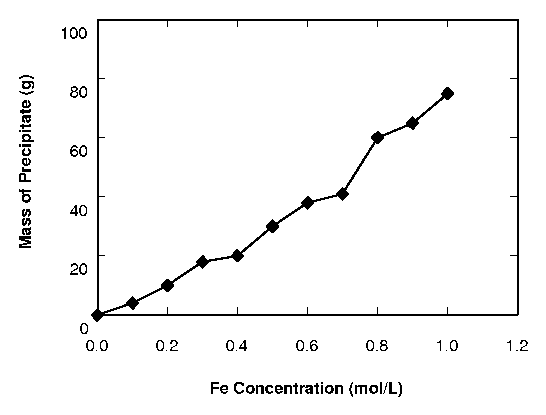
\includegraphics[width=0.48\textwidth]{ISARC_ExampleFigure.eps}
    \caption{Effect of iron concentration on the amount of precipitate formed during hydrolytic precipitation from waste processing solutions}
    \label{fig_1}
\end{figure}

\begin{figure*}[!htb]
    \centering
    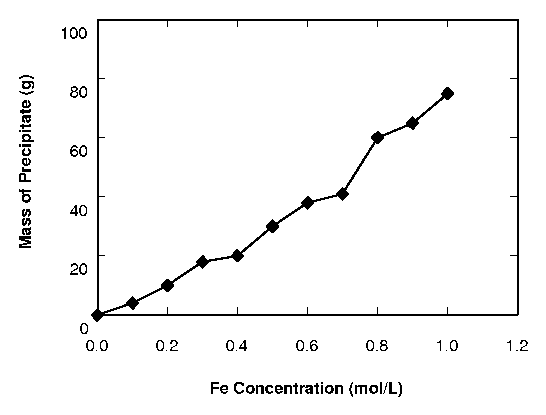
\includegraphics[width=\textwidth]{ISARC_ExampleFigure.eps}
    \caption{Effect of iron concentration on the amount of precipitate formed during hydrolytic precipitation from waste processing solutions}
    \label{fig_2}
\end{figure*}


\subsection{Tables}

Tables should appear as close as possible to their first citation. 
They should be numbered consecutively using Arabic numerals and their title should be centered above the table.

The caption should be formatted with the word `Table ' followed by a character space, the table number, a period, another character space, and the title. 
Separate each table from the adjacent text with one blank line.
See Table~\ref{tab_1} for example.

Table-wide lines (horizontal 0.5 point thickness) separate the title from the column headings, the column headings from the body of the table, and the table from the following text. 
Avoid vertical lines and avoid the use of horizontal lines between the various rows of data.
Text in the tables should have a size not larger than the main text.
Table~\ref{tab_1} shows a good example.

A table too wide to fit in one column may be placed across the width of the page (i.e. between the margins) by using the environment \verb|table*|. 
A table too wide to fit between the margins may be placed in landscape orientation (sideways format), on a page by itself, with the bottom of the figure to the right of the page.
To achieve this, embed the environment \verb|table| within an environment \verb|landscape|.

\begin{table}[!htb]
    \centering
    \caption{Electron microprobe analyses of sphalerite grains in the Kidd Creek ``C'' concentrate}
    \label{tab_1}
    \begin{tabular}{ccc}
    \hline
    Element & Average(wt \%) & Range(wt\%)\\
    \hline
    Zn	&60.8	&59.6 - 63.3\\
    Fe	&5.82	&3.54 - 6.95\\
    Cd	&0.30	&0.12 - 0.42\\
    S	&3.31	&33.6 - 33.5\\
    \hline
    \end{tabular}
\end{table}


\subsection{Cross-referencing headings, numbered equations, figures and tables}

Refer to a figure as `Figure X', not using its relative position.
For achieving this effectively, use the command \verb|\label{}| within the environment \verb|figure| to label each figure, and then use the command \verb|\ref{}| in the text to refer to the label.

The same guidance applies to Tables and Equations, as well as Headings.
In the case of headings, the command \verb|\label{}| must be declared right after the heading commands (e.g. after the command \verb|\section{}|).

Note that all the figures, tables, equations and the main headings in this template all have a label and are referred to in the text using the command \verb|\ref{}|.


\subsection{References}

References to the literature should be cited in the main text with an Arabic number in square brackets \cite{Ha_2012}. 
References should then appear in cited order at the very end of your paper in the Section \textbf{References}. 
Start each reference on a new line with its number in square brackets \cite{Ha_2012}. 
Citation formats are given below for: a journal article \cite{Ha_2012}, conference paper \cite{Kwok_2012}, book \cite{Book}, and a website \cite{Website}.

The formatting of the references is done automatically by the \hologo{LaTeX} template.
All you need to do is add your references in the ISARC.bib Bibtex file and cite the papers in the text using the command \verb|\cite{}| (as well as \verb|\citet{}|).

Within the Bibtex file, please ensure that all references that have a DOI actually include it. It will then appear in the compiled references.



\section{Conclusion}
\label{sec:Conclusion}

We thank you for considering using this \hologo{LaTeX} template for preparing your ISARC paper. 
Using \hologo{LaTeX} helps producing manuscripts that are formatted correctly first time, and thus avoid rework to you and the editorial team. 

If you have any question about the template and its guidelines, do not hesitate to contact the ISARC conference team.


\bibliography{ISARC}

\end{document}
